% Copyright (c) 2023, Adam McKellar & Kai Rothe
% All rights reserved.
%
% This work is licensed under the Creative Commons Attribution 4.0 International License. To view a copy of this license, visit
% http://creativecommons.org/licenses/by/4.0/.

% !TEX engine = luatex
% !TeX spellcheck = en_EN


\documentclass{beamer}

\usepackage{amsmath}
\usepackage{amssymb}

\usepackage{hyperref}
\hypersetup{
	colorlinks,
	allcolors=.,
	urlcolor=blue,
}

\usepackage{fontspec}
\usepackage{polyglossia}
\setmainlanguage{english}

\usepackage{showexpl}

\usepackage[useregional]{datetime2}

% https://hartwork.org/beamer-theme-matrix/
\usetheme{Antibes}
\usecolortheme{beaver}
\useinnertheme{circles}

% pseudocode: 
\usepackage[vlined]{algorithm2e}
\DontPrintSemicolon
\SetKw{KwCont}{continue}

% images:
\usepackage{wrapfig}

\usepackage[
	type={CC},
	modifier={by},
	version={4.0},
	imagemodifier={-80x15},
]{doclicense}


\author{Adam McKellar\qquad Kai Rothe\qquad\quad}
\title{Feedback Arc Set in Tournaments}
\date{June 22, 2023} % date of presentation

\newcommand{\abs}[1]{\left| #1 \right|}

\begin{document}
	\frame{\titlepage}
	
	\begin{frame}{Overview}
		\tableofcontents
		\tiny
		\doclicenseThis
	\end{frame}


	\section{Feedback Arc Set in Tournaments}
	\begin{frame}[fragile]{Feedback Arc Set (FAS)}
		\begin{align*}			
			FAS := \{&(G = (V, E), k) | G \text{ is directed } \\
										&\land \exists E' \subset E : \abs{E'} \leq k : G' = (V, E \setminus E') \text{ is acyclic}  \}		
		\end{align*}
	\end{frame}
	\begin{frame}[fragile]{Feedback Arc Set (FAS) Example}
		Example \(G\) :
		\begin{center}
			\includegraphics<1>[height=0.3\paperheight]{images/FAS/cyclic_graph_example.pdf}
			\includegraphics<2>[height=0.3\paperheight]{images/FAS/cyclic_graph_example_highlight_cycles.pdf}
			\includegraphics<3>[height=0.3\paperheight]{images/FAS/cyclic_graph_example_highlight_solution_k2.pdf}
			\includegraphics<4->[height=0.3\paperheight]{images/FAS/cyclic_graph_example_highlight_solution_k1.pdf}
		\end{center}
		\begin{itemize}
			\item<3-> Solvable for \(k=2\)
			\item<4-> Solvable for \(k=1\)
			\item<5-> \(\Rightarrow (G, 1) \in FAS\)
		\end{itemize}
	\end{frame}

	\begin{frame}[fragile]{Tournaments (T)}
		\begin{center}
			\includegraphics<1>[height=0.3\paperheight]{images/T/complete_graph_example.pdf}
			\includegraphics<2->[height=0.3\paperheight]{images/T/tournament_example.pdf}
		\end{center}
		\begin{itemize}
			\item<1-> Take a complete graph.
			\item<2-> Assign every edge a direction.
			\item<3-> \(T := \{ (G = (V, E)) | \forall u, v \in V : (u, v) \in E \veebar (v, u) \in E \}\)
		\end{itemize}
	\end{frame}
	\begin{frame}[fragile]{Feedback Arc Set in Tournaments (FAST)}
		\[	FAST := \{ (G = (V, E), k) | G \in T \land (G, k) \in FAS \} \]
		\begin{center}
			\includegraphics<2>[height=0.3\paperheight]{images/T/tournament_example.pdf}
			\includegraphics<3->[height=0.3\paperheight]{images/FAST/fast_example.pdf}
		\end{center}
		\begin{itemize}
			\item<3-> \((G, 1)\in FAST\)
		\end{itemize}
	\end{frame}


	\section{Lemma 2.5 (without proof)}
	\begin{frame}[fragile]{Lemma 2.5}
		For a directed graph \(G\)
		\[ G \text{ is acyclic } \Leftrightarrow \underbrace{\bigvee_< \forall (u,v) \in E(G) : u < v}_\text{exists a topological order} \]
		\begin{center}
			\includegraphics<2-3>[height=0.3\paperheight]{images/Lemma25/acyclic_graph.pdf}
			\includegraphics<4->[height=0.3\paperheight]{images/Lemma25/cyclic_graph.pdf}
		\end{center}
		
		\only<3>{ \(V = \{a, b, c, d\}\) \qquad \(E = \{(a, b), (b, c), (c, d), (a, d)\}\) \\
			\(\Rightarrow a < b \land b < c \land c < d \land a < d \Rightarrow a < b < c < d \Rightarrow \text{ acyclic}\)	}
	
		\only<5->{ \(V = \{a, b, c, d\}\) \qquad \(E = \{(a, b), (b, c), (c, d), \color{red} (d, a) \color{black} \}\) \\
			\(\Rightarrow a < b \land b < c \land c < d \land \color{red} d < a \color{black} \Rightarrow a < d \land  \color{red} d < a \color{black} \Rightarrow \text{ no total order } \Rightarrow \text{ cyclic }\) }
	\end{frame}
	

	\section{Observation 2.6}
	\begin{frame}[fragile]{\(\circledast\)}
		\begin{center}
			\includegraphics<1>[height=0.3\paperheight]{images/CircledAsterix/graph_G.pdf}
			\includegraphics<2>[height=0.3\paperheight]{images/CircledAsterix/edges_f.pdf}
			\includegraphics<3>[height=0.3\paperheight]{images/CircledAsterix/edges_revF.pdf}
			\includegraphics<4>[height=0.3\paperheight]{images/CircledAsterix/graph_GrevF.pdf}
		\end{center}
		\begin{itemize}[<+->]
			\item \(G = (V, E)\)
			\item \(F \subseteq E(G)\)
			\item \(rev(F) := \{(u, v) : (v, u) \in F\}\)
			\item \large \[ G\circledast F := \left( V(G), \left( E(G) \setminus F \right) \cup rev(F) \right)  \]
		\end{itemize}
	\end{frame}

	\begin{frame}[fragile]{Observation 2.6}
		\begin{center}
			\includegraphics<1>[height=0.3\paperheight]{images/Observation26/cyclic_graph_with_F.pdf}
			\includegraphics<2>[height=0.3\paperheight]{images/Observation26/acyclic_G_ast_F.pdf}
			\includegraphics<3>[height=0.3\paperheight]{images/Observation26/acyclic_G_without_FAS.pdf}
		\end{center}
		\only<+->{\[ 
			F \subseteq E(G)	
		\]}
		\only<+->{\[ 
			\text{if } G\circledast F \text{ is a directed acyclic graph}
		\]}
		\only<+->{\[ 
			\Rightarrow F \text{ is a feedback arc set of } G	
		\]}
	\end{frame}
	\begin{frame}[fragile]{Observation 2.6 \textit{ is implied by Lemma 2.5 }}
		\begin{center}
			\includegraphics<1>[height=0.3\paperheight]{images/Observation26/cyclic_graph_with_F.pdf}
			\includegraphics<2>[height=0.3\paperheight]{images/Observation26/acyclic_G_ast_F.pdf}
			\includegraphics<3>[height=0.3\paperheight]{images/Observation26/acyclic_G_without_FAS.pdf}
		\end{center}
		
		\only<1>{ \(V = \{a, b, c, d\}\) \qquad \(E = \{(a, b), (b, c), (c, d), \color{red} (d, a) \color{black} \}\) \\
			\(\Rightarrow a < b \land b < c \land c < d \land \color{red} d < \dotsc \color{black} \Rightarrow \text{ no total order } \Rightarrow \text{ cyclic }\) }
	 	\only<2-3>{\(V = \{a, b, c, d\}\) \qquad \((E\cup rev(F))\setminus F = \{(a, b), (b, c), (c, d), \color{blue}(a, d) \color{black} \}\) \\
			\(\Rightarrow a < b \land b < c \land c < d \land \color{blue} a < d \color{black} \Rightarrow a < b < c < d \Rightarrow \text{ acyclic}\)}
		\only<3>{\[ \Rightarrow   a < b \land b < c \land c < d \Rightarrow a < b < c < d \Rightarrow \text{ acyclic}\]}
		
	\end{frame}
	
	
	\section{Lemma 2.7}
	\begin{frame}[fragile]{\(\min\)}
		\[ \text{for } S \subset \mathcal{P}(E(G)) \]
		\[ \min S := \left\{ M \in S : \forall M' \in S : \abs{M} \leq \abs{M'} \right\} \]
	\end{frame}
	
	\begin{frame}[fragile]{Lemma 2.7}
		\begin{align*}
			&\qquad F \in \min \left\{ F' \subset E(G) | F' \text{ is a Feedback Arc Set of } G \right\} \\
			&\Leftrightarrow \\
			&\qquad F \in \min \left\{ F' \subset E(G) | G\circledast F' \text{ is acyclic} \right\}
		\end{align*}	
	\end{frame}
	
	\subsection{Lemma 2.7 ``\(\Rightarrow\)''}
	\begin{frame}[fragile]{Lemma 2.7 ``\(\Rightarrow\)''}
		\begin{align*}
			&\qquad F \in \min \left\{ F' \subset E(G) | F' \text{ is a Feedback Arc Set of } G \right\} \\
			&\Rightarrow \\
			&\qquad F \in \min \left\{ F' \subset E(G) | G\circledast F' \text{ is acyclic} \right\}
		\end{align*}	
	\end{frame}
	\begin{frame}[fragile]{Lemma 2.7 ``\(\Rightarrow\)'' \--- Assumptions}
		\begin{center}
			\includegraphics<1>[height=0.3\paperheight]{images/Lemma27/Abstract_Graph_G_with_Edge_of_F.pdf}
			\includegraphics<2>[height=0.3\paperheight]{images/Lemma27/Abstract_Graph_G_without_F.pdf}
			\includegraphics<3-5>[height=0.3\paperheight]{images/Lemma27/Abstract_Graph_G_with_Edge_of_revF_and_Cycle_C.pdf}
			\includegraphics<6>[height=0.3\paperheight]{images/Lemma27/Abstract_Graph_G_with_Edge_of_revF_and_Cycle_C_2.pdf}
		\end{center}
		\begin{enumerate}
			\item<1-> \(  F \in \min \left\{ F' \subset E(G) | F' \text{ is a Feedback Arc Set of } G \right\} \)
			\item<2-> \(\Rightarrow G' = \left(V(G), E(G)\setminus F\right) \) is acyclic
			\item<3-> \textbf{Assumption:} \( G\circledast F \) has a cycle \( \color{blue} C \)
			\item<4-> \(\Rightarrow E(C) \cup \left(E(G)\setminus F\right) \neq \left(E(G)\setminus F\right)\)
			\item<5-> \(\Rightarrow \exists f \in E(C) : f\in rev(F)\)
			\item<6-> \( \left\{ f_1, f_2, \dotsc, f_n \right\} = E(C) \cap rev(F) \) in order of their appearance in \(C\) \\
			\quad \( \left\{ e_1, \dotsc , e_n \right\} =  rev( \left\{ f_1, \dotsc, f_n \right\} ) \)			
		\end{enumerate}
	\end{frame}
	\begin{frame}[fragile]{Lemma 2.7 ``\(\Rightarrow\)'' \--- Contradiction}
		\begin{center}
			\includegraphics<1-2>[height=0.3\paperheight]{images/Lemma27/Abstract_Graph_G_with_Edge_of_F_and_Cylce_of_G.pdf}
			\includegraphics<3>[height=0.3\paperheight]{images/Lemma27/Abstract_Graph_G_with_Edge_of_revF_and_Cycle_C_2.pdf}
			\includegraphics<4->[height=0.3\paperheight]{images/Lemma27/Abstract_Graph_G_with_C_and_C_of_i.pdf}
		\end{center}
		\begin{itemize}[<+->]
			\item \(F\text{ is minimal } \Rightarrow \text{ for each } e_i \text{ exists a cycle } C_i \text{ of } G  \) \\
			which is traversable via edges \( (E(G)\setminus F)\cup \{e_i\} \)
			\item \( F \cap E(C_i) = \{e_i\} \)
		\end{itemize}
		\begin{enumerate}[<+->]
		 	\item Traverse \(C\) in \(G\)
		 	\item Instead of traversing \(f_i = rev(e_i)\), we traverse \(C_i - e_i\)
		 	\item \(C\) can be traversed without edges of \(rev(F)\) or \(F\)
		 	\item \textbf{Contradiction!} \(G' = \left(V(G), E(G)\setminus F\right)\) has a cycle!
		\end{enumerate}
	\end{frame}
	\begin{frame}[fragile]{Lemma 2.7 ``\(\Rightarrow\)'' \--- F is Minimal}
		\begin{itemize}[<+->]			
			\item We have shown:
			\begin{align*}
				&\qquad F \in \min \left\{ F' \subset E(G) | F' \text{ is a Feedback Arc Set of } G \right\} \\
				&\Rightarrow \\
				&\qquad G\circledast F \text{ is acyclic}
			\end{align*}
		
			\item We still need to show:
			\begin{align*}
				&\qquad F \in \min \left\{ F' \subset E(G) | F' \text{ is a Feedback Arc Set of } G \right\} \\
				&\Rightarrow \\
				&\qquad F \in \min \left\{ F' \subset E(G) | G\circledast F' \text{ is acyclic} \right\}
			\end{align*}
		\end{itemize}	
	\end{frame}
	\begin{frame}[fragile]{Lemma 2.7 ``\(\Rightarrow\)'' \--- F is Minimal \--- Proof}
		\only<1->{
			\begin{align*}
				\text{let \quad} &F \in \min \left\{ F' \subset E(G) | F' \text{ is a Feedback Arc Set of } G \right\} \\
				\text{if \quad} &F \notin \min \left\{ F' \subset E(G) | G\circledast F' \text{ is acyclic} \right\}
			\end{align*}
		}
		\only<2->{\[ \Rightarrow F'' \in \min \left\{ F' \subset E(G) | G\circledast F' \text{ is acyclic} \right\} \]}
		\only<3->{\[ \Rightarrow \abs{F''} < \abs{F} \]}
		\only<4->{\[ G\circledast F'' \text{ is acyclic } \stackrel{\text{Observation 2.6}}{\Rightarrow} F'' \text{ is a feedback arc set of } G  \]}
		\only<5->{\[ \Rightarrow F \notin  \min \left\{ F' \subset E(G) | F' \text{ is a Feedback Arc Set of } G \right\} \]}
		\only<6->{\textbf{Contradiction!}}
	\end{frame}
	
	
	\subsection{Lemma 2.7 ``\(\Leftarrow\)''}
	\begin{frame}[fragile]{Lemma 2.7 ``\(\Leftarrow\)''}
		\begin{align*}
			&\qquad F \in \min \left\{ F' \subset E(G) | F' \text{ is a Feedback Arc Set of } G \right\} \\
			&\Leftarrow \\
			&\qquad F \in \min \left\{ F' \subset E(G) | G\circledast F' \text{ is acyclic} \right\}
		\end{align*}
	\end{frame}
	\begin{frame}[fragile]{Lemma 2.7 ``\(\Leftarrow\)'' \--- Proof}
		\only<+->{\[ F \in \min \left\{ F' \subset E(G) | G\circledast F' \text{ is acyclic} \right\} \]}
		\only<+->{\[ \stackrel{\text{Observation 2.6}}{\Rightarrow} F \text{ is a Feedback Arc Set of } G \]}
		\only<+->{\[ \text{if } \exists F''\subsetneq F : F''\in \min \left\{ F' \subset E(G) | F' \text{ is a FAS of } G \right\} \]}
		\only<+->{\[ \Rightarrow \exists F'' : \left( \abs{F''} < \abs{F} \right) \land \left( F'' \in \min \left\{ F' \subset E(G) | F' \text{ is a FAS of } G \right\} \right) \]}
		\only<+->{\[ \stackrel{\text{Lemma 2.7 } \Rightarrow}{\Rightarrow} F'' \in \min \left\{ F' \subset E(G) | G\circledast F' \text{ is acyclic} \right\} \]}
		\only<+->{\textbf{Contradiction!}}
	\end{frame}

	\begin{frame}[fragile]{Transition}
		\begin{flalign*}
			&\qquad G\circledast F \text{ is a directed acyclic graph} &\\
			&\stackrel{\text{\textbf{Observation 2.6}}}{\Rightarrow} &\\
			&\qquad F \text{ is a feedback arc set of } G &
		\end{flalign*}	
		\begin{flalign*}
			&\qquad F \in \min \left\{ F' \subset E(G) | F' \text{ is a Feedback Arc Set of } G \right\} &\\
			&\stackrel{\text{\textbf{Lemma 2.7}}}{\Leftrightarrow} &\\
			&\qquad F \in \min \left\{ F' \subset E(G) | G\circledast F' \text{ is acyclic} \right\} &
		\end{flalign*}
	\end{frame}
	
	
		\section{Theorem 2.8: quadratic kernel for feedback arc sets in tournaments}
	\begin{frame}[fragile]{Theorem 2.8}
		\textit{FAST} admits a kernel with at most \(k^{2} + 2k\) vertices. \newline 
		\newline
		\only<2->{ There is an algorithm returning in \textit{polynomial} time \((G',k')\): }
		\begin{itemize}
			\item<3-> \((G,k) \in FAST \Leftrightarrow (G', k') \in FAST \)
			\item<4-> \(\abs{V(G')}\le k^2 + 2k \)
		\end{itemize}
	\end{frame}
	
	\begin{frame}[fragile]{Triangle}
		A \textit{triangle} is a directed cycle of length three. 
		\begin{center}
			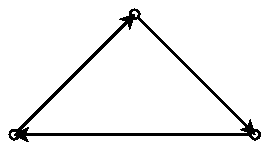
\includegraphics[height=0.3\paperheight]{images/Triangle/Triangle.pdf}
		\end{center}
		% \uncover<2->{
		% \begin{align*}
		%	\Delta_{G} := \{& (e_1, e_2, e_3) \in E(G)^3 | \\
		%	 		       & \exists v_1 \neq v_2 \neq v_3 \in V(G): \\
		%			       & e_1 = (v_1, v_2) \land e_2 = (v_2, v_3) \land e_3 = (v_3, v_1) \} 
		% \end{align*} 
		% }
	\end{frame}
	
	\begin{frame}[fragile]{Reduction FAST.1}
		If an edge \(e\) is contained in at least \(k+1\) triangles, then reverse \(e\) and reduce \(k\) by \(1\). \newline 
		
		\begin{center}
		\uncover<2->{ 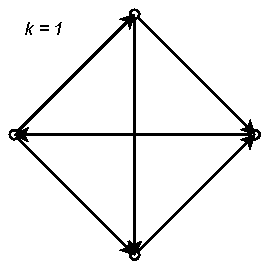
\includegraphics[height=0.5\paperheight]{images/FAST_1/Triangle2.pdf} }
		\uncover<3>{ 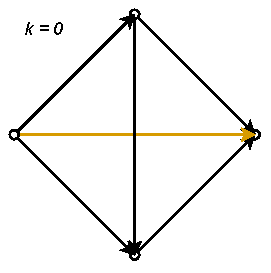
\includegraphics[height=0.5\paperheight]{images/FAST_1/Triangle2Rev.pdf} }
		\end{center}
	\end{frame}
	
	\begin{frame}[fragile]{Reduction FAST.1 - Safeness}
		Let $(G, k)$ be an instance of FAST. If there is an edge $e \in E(G)$ contained at least $k+1$ triangles, then $e \in F$ for every Feedback Arc Set $F \subset E(G)$ with $\abs{F} \leq k$. 
		
		\begin{center}
			\includegraphics<2>[height=0.6\paperheight]{images/FAST_1/FAST1_Safeness1.pdf}
			\includegraphics<3>[height=0.6\paperheight]{images/FAST_1/FAST1_Safeness2.pdf}
		\end{center}
	\end{frame}
	
	\begin{frame}[fragile]{Reduction FAST.1 - Safeness}
		\textit{Proof:} Let $(G, k)$ be an instance of FAST. If there is an edge $e \in E(G)$ contained at least $k+1$ triangles, then $e \in F$ for every Feedback Arc Set $F \subset E(G)$ with $\abs{F} \leq k$. 
		\begin{itemize}
		 \item If an edge $e = (u, v)$ is contained in triangle $t$, then $t$ is determined by its third vertex $w_t$, s.t. $(u, v), (v, w), (w, u) \in t$. 
		 \item If an edge $e$ is contained in two different triangles $t_1 \neq t_2$, then $w_{t_1} \neq w_{t_2}$ and thus not other edge except $e$ is contained in both triangles.
		 \item Assume there is an edge $e$ contained in at least $k+1$ triangles. If there is a Feedback Arc Set $F \subset E(G)$  with $e \notin F$ and $\abs{F} \leq k$, for each of the at least $k+1$ triangles at least one edge is in $F$. Since all those edges are (pairwise) different, $\abs{F} \geq k+1$. A Contradiction!
		\end{itemize}
	\end{frame}
	
	\begin{frame}[fragile]{Reduction FAST.1 - Polynomial time}
		\begin{algorithm}[H]
		\only<1>{
		\KwData{\( (G, k) \) instance of FAST}
		\KwResult{\( (G', k') \) reduced instance of FAST}
		\BlankLine
		}
		\only<1>{
		$\Delta := \{ \}$\;
		\For{$e_1 = (u_1, v_1) \in E(G)$}{
			\For{$e_2 = (u_2, v_2) \in E(G) \setminus \{e_1\}$}{
				\For{$e_3 = (u_3, v_3) \in E(G) \setminus \{e_1, e_2\}$}{
					\If{$(e_1, e_2, e_3)$ is a triangle, i.e. $v_1 = u_2, v_2 = u_3, v_3 = u_1$}{
						put $(e_1, e_2, e_3)$ in $\Delta$\;
					}
				}
			}
		}
		... \;
		}
		\only<2->{
		... \;
		% $\Delta = \{(e_1, e_2, e_3) \in E(G)^3 | \exists v_1 \neq v_2 \neq v_3 \in V(G): e_1 = (v_1, v_2) \land e_2 = (v_2, v_3) \land e_3 = (v_3, v_1) \} $\;
		\BlankLine	
		\For{$e \in E(G)$}{
			$counter := 0$\;
			\For{$t \in \Delta$}{
				\If{$e \in t$}{$counter \gets counter + 1$\;}
				\If{$counter \geq k+1$}{\KwRet{$(G \circledast \{e\}, k-1)$}\;}
			}
		}
		\KwRet{$(G,k)$}\;
		}
		\end{algorithm}
		\uncover<3->{
		\bigskip
		$\Rightarrow$ FAST.1 is computable in polynomial time, e.g. bounded by
		\[ \mathcal{O}(\abs{E(G)}^3) + \mathcal{O}(\abs{E(G)}^4) = \mathcal{O}(\abs{E(G)}^4) \]
		}
	\end{frame}
	
	\begin{frame}[fragile]{Reduction FAST.2}
		If a vertex \(v\) is not contained in any triangle, then delete \(v\) from the tournament.
		\begin{center}
		\uncover<2->{ 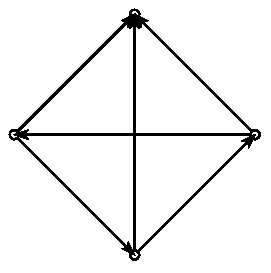
\includegraphics[height=0.5\paperheight]{images/FAST_2/GraphWithVertexUncolored.pdf} }
		\uncover<3->{ 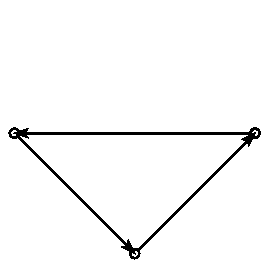
\includegraphics[height=0.5\paperheight]{images/FAST_2/GraphWithoutVertex.pdf} }
		\end{center}
	\end{frame}
	
	\begin{frame}[fragile]{Reduction FAST.2 - Safeness}
		If a vertex \(v\) of a tournament is contained in a circle of length $L > 3$, then $v$ is also contained in a circle of length $L' < L$.
		\begin{center}
		\includegraphics<2>[height=0.6\paperheight]{images/FAST_2/FAST2_Safeness1.pdf}
		\includegraphics<3>[height=0.6\paperheight]{images/FAST_2/FAST2_Safeness2.pdf} 
		\includegraphics<4>[height=0.6\paperheight]{images/FAST_2/FAST2_Safeness3.pdf} 
		\end{center}
	\end{frame}
	
	\begin{frame}[fragile]{Reduction FAST.2 - Safeness}
		\textit{Proof:} Let $(G, k)$ be an instance of FAST. If a vertex \(v \in V(G)\) is not contained in triangle, then $v$ is not contained in a directed circle.		\begin{itemize}
		\item If a vertex  \(v \in V(G)\) is contained in a directed circle, then $v$ is contained in a triangle. This follows from repeated application of the following argument:
		\item Let $v$ be contained in a directed circle $v, w_1, w_2, ..., w_{L-1}$. If $L = 3$ finish. Since $G$ is a tournament, else $L > 3$ and either $(v, w_2) \in E(G)$ or $(w_2, v) \in E(G)$.
		\item If $(v, w_2) \in E(G)$, then $v, w_2, ..., w_{L-1}$ are contained in a directed circle of length $L' = L-1 < L$.
		\item If  $(w_2, v) \in E(G)$, then $v, w_1, w_2$ are contained in a triangle of length $L' = 3 < L$.
		\item Thus $v$ is also contained in a directed circle of length $L' < L$. 
		\end{itemize}
	\end{frame}
	
	\begin{frame}[fragile]{Reduction FAST.2 - Polynomial time}
		\begin{algorithm}[H]
		\only<1>{
		\KwData{\( (G, k) \) instance of FAST}
		\KwResult{\( (G', k') \) reduced instance of FAST}
		\BlankLine
		}
		\only<1>{
		$\Delta := \{ \}$\;
		\For{$e_1 = (u_1, v_1) \in E(G)$}{
			\For{$e_2 = (u_2, v_2) \in E(G) \setminus \{e_1\}$}{
				\For{$e_3 = (u_3, v_3) \in E(G) \setminus \{e_1, e_2\}$}{
					\If{$(e_1, e_2, e_3)$ is a triangle, i.e. $v_1 = u_2, v_2 = u_3, v_3 = u_1$}{
						put $(e_1, e_2, e_3)$ in $\Delta$\;
					}
				}
			}
		}
		... \;
		}
		\only<2->{
		... \;
		% $\Delta = \{(e_1, e_2, e_3) \in E(G)^3 | \exists v_1 \neq v_2 \neq v_3 \in V(G): e_1 = (v_1, v_2) \land e_2 = (v_2, v_3) \land e_3 = (v_3, v_1) \} $\;	
		\BlankLine			 
		\For{$v \in V(G)$}{
			\For{$t \in \Delta$}{
				\If{$v \in t$}{skip $v$\;}
			}
			\KwRet{$(G-v,k)$}\;
		}
		\KwRet{$(G,k)$}\;
		}
		\end{algorithm}
		\uncover<3->{
		\bigskip
		$\Rightarrow$ FAST.2 is computable in polynomial time, e.g. bounded by
		\[ \mathcal{O}(\abs{E(G)}^3) + \mathcal{O}(\abs{V(G)} \cdot \abs{E(G)}^3) + \mathcal{O}(\abs{E(G)}) = \mathcal{O}(\abs{V(G)} \cdot \abs{E(G)}^3) \]
		}
		\end{frame}
		
	\begin{frame}[fragile]{Theorem 2.8 - Upper Size Bound}
		Let \((G,k) \in FAST\) : neither FAST.1 nor FAST.2 are applicable. 
		\begin{center}
		\includegraphics<2>[height=0.25\paperheight]{images/Theorem28/Theorem28_5.pdf}
		\includegraphics<3>[height=0.35\paperheight]{images/Theorem28/Theorem28_4.pdf}
		\includegraphics<4>[height=0.4\paperheight]{images/Theorem28/Theorem28_3.pdf}
		\includegraphics<5>[height=0.25\paperheight]{images/Theorem28/Theorem28_2.pdf}
		\includegraphics<6->[height=0.35\paperheight]{images/Theorem28/Theorem28_1.pdf}
		\end{center}
		\only<7> { \[ \Rightarrow \abs{V(G)} \leq k(k+2) \] }
		
	\end{frame}
	
	\begin{frame}[fragile]{Theorem 2.8 - Upper Size Bound}
		\textit{Proof:} If \((G,k) \in FAST\) such that neither FAST.1 nor FAST.2 are applicable, then $\abs{V(G)} \leq k(k+2)$. 
		\begin{itemize}
		 \item Every vertex $v \in V(G)$ must be contained in a triangle $t$, else FAST.2 could be applied. 
		 \item Since \((G,k) \in FAST\), there is a Feedback Arc Set $F \subset E(G)$ with $\abs{F} \leq k$. Then for every triangle $t$ there is at least one edge $e \in t$ in $F$.
		 \item Every edge $e \in F$ is contained in at most $k$ triangles, else FAST.1 could be applied. Thus for each edge $e \in F$ there are at most $k+2$ vertices contained in a triangle with $e$. 
		\item Since all vertices $v$ are contained in a triangle with an edge $e \in F$, and there are at most $k$ edges in $F$, there are at most $k(k+2)$ vertices in $G$.
		\end{itemize}
	\end{frame}
	
	% Define recursive Function for pseudocode
	\RestyleAlgo{ruled}
	\begin{frame}[fragile]{Theorem 2.8 - FAST Kernel}
	\begin{function}[H]
		\caption{Kernel(G, k)}
		\KwData{\( (G, k) \) instance of FAST}
		\KwResult{\( (G', k') \) reduced instance of FAST}
		\BlankLine
		\If{$ k > 0 \land (G',k') =$ FAST.1$(G,k) \neq (G,k)$}{Kernel(G',k')}
		\If{$(G',k') =$ FAST.2$(G,k) \neq (G,k)$}{Kernel(G',k')}
		\If{$\abs{V(G)} > k(k+2)$}{\KwRet{No-Instance $(G', k')$ with $\abs{V(G')} \leq k'(k'+2)$}}
		\KwRet{$(G,k)$}
	\end{function}
	\uncover<2->{
	\bigskip
	$\Rightarrow$ FAST Kernel computable in polynomial time, e.g. bounded by
	\[ \mathcal{O}( (k + \abs{V(G)}) \cdot (\abs{E(G)}^3 + \abs{V(G)} \cdot \abs{E(G)}^3) ) \]
	}
	
	\end{frame}
	
	\begin{frame}[fragile]{Theorem 2.8}
		\textit{FAST} admits a kernel with at most \(k^{2} + 2k\) vertices. \newline 
		\newline
		There is an algorithm returning in \textit{polynomial} time \((G',k'): \)
		\begin{itemize}
			\item \((G,k) \in FAST \Leftrightarrow (G', k') \in FAST \)
			\item \(\abs{V(G')} \leq k(k+2) = k^2 + 2k \)
		\end{itemize}
	\end{frame}
	
\end{document}